\chapter{Introduction}
\label{chp:introduction}
After the introduction of the Internet on 60's and world wide web on 90's, there are more and more people connected each other using this technology. Initially, the architecture used to build the Internet is Peer-to-peer network although the most popular one is \textit{client and server}. A \textit{server} holds the content and delivers it to a user at the \textit{client} side, thus burden the server. Currently, recent research shows that peer-to-peer Internet already back at its prime by dominating the traffic\cite{2015:internettraffic:sandvine}.

Interaction among user in the Internet community can be expressed in various fashion. Peer-to-peer (P2P) is one of the major interaction existed in the net. This shown in figure \ref{fig:usage}. Many applications and protocols run on top of P2P system, online gaming, computing, and the most popular one, file sharing. \bt~is by far the most popular system used in file-sharing community with its unique \textit{tit-for-tat} mechanism to discourage uncooperative peers \cite{2003:bittorrent:cohen}. 

\begin{figure}[h]
	\centering
	\begin{subfigure}[b]{0.8\textwidth}
		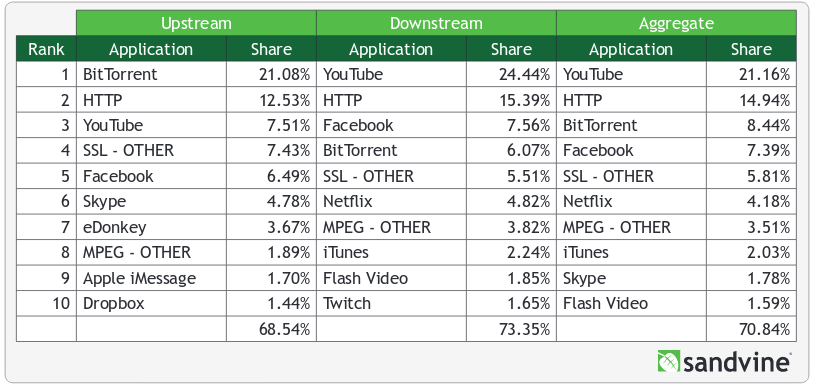
\includegraphics[width=\linewidth]{pics/sandvineeu2015}
		\caption{Sandvine data for 2015 internet usage in Europe}
		\label{fig:usage1}
	\end{subfigure}\\
	\begin{subfigure}[b]{0.8\textwidth}
		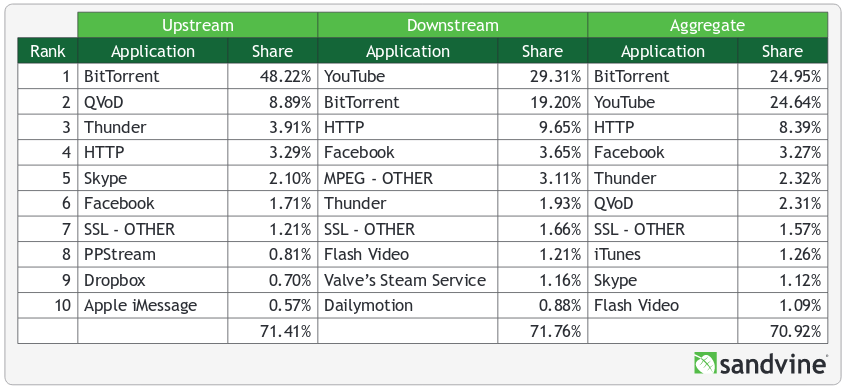
\includegraphics[width=\linewidth]{pics/sandvineasia2015}
		\caption{Sandvine data for 2015 internet usage in Asia Pasific}
		\label{fig:usage2}
	\end{subfigure}%
	\caption{Traffic of the Internet by Sandvine \cite{2015:internettraffic:sandvine}}.
	\label{fig:usage}
\end{figure}

Peer-to-peer network has many different applications. Some of them are multimedia streaming, online gaming, and file-transfer. All of those applications has different requirement to ensure user has flawless experience. Multimedia streaming, for example, need to achieve two conditions. First, the start up delay must be small to make sure user do not abandon his intent to stream the files. Secondly, the chunk (or piece) loss must be negligible, or at least low enough to provide good quality\cite{2008:givetogetvod:Mol}. Other application, P2P gaming, require more complex situation. Depend on the type of the game (e.g., FPS), peer latency must be under certain threshold\cite{2010:surveyp2pgame:shen}. It also needs to consider bandwidth demand and high security to prevent cheating between user. The most common P2P application, file transfer, obviously need high throughput by maximizing all the connection a user has.

\section{The arise of freeriding}
Among all the peer-to-peer usage in the Internet, file-sharing is the most popular one. It started with Napster in 1999 to share music file between its users. It shut down at 2001 and immediately followed by Kazaa and Gnutella afterward. Both services allowed the user to share not only music file but also another type of files. Currently, both already shut down because of legal and performance issues. In Gnutella case, majority of users (70\%) stopped to share their files. Moreover, about half of the communication only served by top 1\% of the community \cite{2000:freeridegnutella:adar}. Gnutella suffers from a social phenomenon called \textit{freeriding} on majority of its users.

Freerider, can cause several problems, especially in peer-to-peer network. First and foremost, freeriding behaviour can lead to vulnerabilities in the system. With only few of the user provide the service for many, it is eventually become more centralized than decentralized system. Another well known problem caused by freeriders is the degradation of system performance \cite{2000:freeridegnutella:adar}. If freeriders become majority in file-sharing peer-to-peer system, as they occupy significant amount of resource, eventually bottleneck in the system will occur. As the time goes, honest peer may not feel satisfied and decided to leave the system. With important peer leave the system, it will degrade more and lost the file that used to be served by leaving peer. The system become unhealthy and sooner or later will be completely left by its peers.

If everyone can free ride, the whole system performance may degrade significantly. In other words, freeriding can lead to systematically worse problem called ``tragedy of the commons'' \cite{1968:tragedycommon:hardin}. This problem is popularized by \citet*{1968:tragedycommon:hardin} in \citeyear{1968:tragedycommon:hardin}. This social dilemma emerge because overuse and overexploitation in the shared resource without feedback from the user. 
% how can egoist cooperate :  The Emergence of Cooperation among Egoists (Robert Axelrod). Solved by tit-for-tat -> good performance. managing supply and demand meulpowder p.7

% freerider behaviour, tit-for-tat result
In \bt, one of the protocol used in file-sharing, it is unlikely a user will extremely freeride. We define this behavior as not upload anything while keep downloading data. Instead of extremely freeriding, it is more common to find \textit{hit and run} behavior \cite{2011:managesupplydemand:meulpolder}. Hit and run (HnR) is a situation where a user has finished downloading then immediately stop his contribution. Hit and run also often referred as one of the freeriding behavior that peer-to-peer community wanted to prevent. \citeauthor{2015:freeriderinbtcommunity:das} also studied the freerider behavior in \bt~communities. They conclude that freerider in \bt~may not degrade performance as long as the swarm has at least one dedicated and available seeders. The potential availability of seeder also become a factor that keeping the swarm alive \cite{2015:freeriderinbtcommunity:das}. 
%. One thing that need to take into consideration is that in their research, they only take four communities as dataset 

\section{BitTorrent protocol}
\bt~\cite{2003:bittorrent:cohen}, nowadays, stand as \textit{de facto} file-sharing protocol on top of peer-to-peer network. It survives until now because \bt~ is a \textit{protocol} that can be implemented by anyone, instead of service that Napster, Kazaa, and Gnutella used to have. To build \bt~environment, it is essential to know the complete view how \bt~work. 

% tit-for-tat, choking, unchoke, optimistic unchoke
In general view, \bt~consists of peers who participated in file-sharing and \textit{tracker}. \textit{Tracker} is responsible for monitors the distribution and progress of the file and peers in the swarm. \textit{Swarm} is a set of peers formed with the same purpose of downloading or uploading certain files represented in \texttt{.torrent} metadata file. Static \texttt{.torrent} file, which contains information such as tracker addresses and unique hash value of this swarm, is created by peer who wants to publish their files. Peer uses information in \texttt{.torrent} file to connect each other. Files in a swarm consists of several \textit{chunks} or file pieces. A chunk is exchanged by the peers in a particular \textit{session}. A peer actively participated in many swarms on the uninterrupted time-frame called \textit{session}. 

In \bt, it is desirable to have many peers upload piece of file to the swarm. This way, swarm can be \textit{healthier}, and overall download speed can increase. However, many peers become a \textit{leecher}, which quit the swarm when his download finished. This behavior also called as \textit{Hit and Run} (HnR) \cite{2014:sustainabilitytorrent:chen}. In general, those unwanted behavior normally forbidden in so-called \textit{private communities}. In such a community, the administrator enforces several policy such as \textit{Share Ratio Enforcement} (SRE). SRE define the amount a user need to upload before able to download from the community \cite{2012:economicbt:kash}. 

% how bittorrent handle freeriding (short term)
\bt~uses \textit{tit-for-tat} mechanism to reward good behavior and punish bad behavior. This mechanism tried to solve fairness issue introduced by freeriding behavior \cite{2003:bittorrent:cohen}. \textit{Tit-for-tat} in \bt~ encourage user to only upload file to one who also has uploaded his file somewhere else. Furthermore, it is also ranked by upload amount and speed. Freerider always getting low priority in this mechanism. In this way, \textit{tit-for-tat} incentivizes for user to upload a file. \bt~protocol and its \textit{tit-for-tat} become a standard in file-sharing peer-to-peer system with many clients implemented this protocol. \textit{Tit-for-tat} valid only in a scope of single torrent. That means, the configuration from one community can not be carried to another community. This causes \textit{tit-for-tat} works best only in short term transaction and limited parties.

\textit{Tit-for-tat} is a distinguished feature to force cooperation of other peers. By peers reciprocation, \bt~ implement \textit{choking algorithm} under this feature. It is basically prioritize peer who provided high upload rates. Choking algorithm is an algorithm to temporarily refuse uploading piece of file to a particular peer. Usually, an uploader has a limited number of unchoked slots. By observing other peers, choking algorithm decides which peer a particular piece will be sent or not sent to. If we unchoke a peer, it means we consider to upload a piece to that peer. For starters, it is usually useful to execute \textit{optimistic unchoking} \cite{2003:bittorrent:cohen}. Optimistic unchoking is an algorithm to unchoke a peer regardless of its activity in a swarm. This gives a peer a chance to increase his upload rate by providing more content. As for downloading, a peer picks \textit{rarest-first} chunk based on the availability in the swarm. This technique make sure that a complete file is distributed in the swarm.

%\todo{expand_:Delivery procedure} -> 



\subsection{Tribler}
Tribler\footnote{\url{https://www.tribler.org/}} is peer-to-peer file sharing application developed at Delft University of Technology that compatible with \bt~protocol \cite{2008:tribler:pouwelse}. Tribler focused on security, fully decentralized system, and anonymity. Starts with ABC (Another \bt~Client), Tribler currently provides content discovery, channels concept, and reputation management in fully distributed manner. With Tribler downloaded from the official repository on the latest stable release (6.5.2) reaching  78440\footnote{\url{http://www.somsubhra.com/github-release-stats/ ?username=tribler&repository=tribler} (Accessed 3 September 2016)} times, it is desired to observe the usage of CMS with an adequate user base. We believe our work will be able to increase the overall swarm throughput by donating unused bandwidth on peer upstream.

All of the Tribler main components such as end-to-end encryption, channel discovery, and many others relied in database and dissemination system called \texttt{Dispersy} \cite{2013:dispersy:zeilemaker}. Dispersy maintain and perform the communication between Tribler peers in fully decentralized manner. Dispersy able to circulate the message in one-to-one or one-to-many within a group of node called \texttt{community}. User can adapt and implement its desired \textit{community} by itself. It is including how, what, and where the communication will occur.

Tribler implements several Dispersy \textit{communities} on its core function. \citeauthor{2016:tribler-techdebt:vos} summarize the recent community in Tribler. Important features such as channel discovery, search within community, end-to-end Tor-like operations, and currency mechanism shown in table \ref{tbl:community}. \textit{Channel} is a collection of torrent that has extra capabilities such as vote system, spam prevention, and comment (social) attributes. Every user can create his own channel, add and remove torrent to it, and maintain its activity. Worth to mention that Tribler implemented its own reputation system to incentivize user. Reputable user will get boost from other Tribler user, so it is beneficial in its own way.

In Tribler, there were several attemps to tackle freerider issue. Give-to-Get \cite{2008:givetogetvod:Mol} is one approach in peer-to-peer streaming video system. It works by give freerider only idle bandwidth slots and therefore their download speed will much slower\footnote{\url{https://www.tribler.org/Give-To-Get/}(Accessed 22 September 2016)}. There was also reputation management implemented in \textit{BarterCast4 community}, specifically to prevent freeriding in Tribler \cite{2009:bartercast:meulpolder}. It was used to spread the statistics about upload and download rate of a particular user \cite{2016:tribler-techdebt:vos}. And lastly, there is Multichain \cite{2015:multichain:norberhuis}, the anonymous tamper-proof interaction history that works on onion routing in Tribler network. The relation between MultiChain and BarterCast4 will be discussed in section \ref{section:sec_currency}.

\begin{table}[tbp]
	\centering
	\caption{Overview of implemented Dispersy community in Tribler \cite{2016:tribler-techdebt:vos}.}
	\label{tbl:community}
	\begin{tabular}{|l|p{11cm}|}
		\hline
		\rowcolor[HTML]{EFEFEF} 
		\multicolumn{1}{|c|}{\cellcolor[HTML]{EFEFEF}{\color[HTML]{333333} \textbf{Community Name}}} & \multicolumn{1}{c|}{\cellcolor[HTML]{EFEFEF}{\color[HTML]{333333} \textbf{Purpose}}}                                                                                                                                     \\ \hline
		\textit{AllChannel}                                                                          & Used to discover new channels and to perform remote channel search operations.                                                                                                                                           \\ \hline
		\textit{BarterCast4}                                                                         & While currently disabled, this community was used to spread statistics about the upload and download rates of peers inside the network and has originally been created as a mechanism to prevent free-riding in Tribler. \\ \hline
		\textit{Channel}                                                                             & This community represents a single channel and is responsible for managing torrents and playlists inside that channel.                                                                                                   \\ \hline
		\textit{Multichain}                                                                          & This community utilizes the blockchain technology and can be regarded as the accounting mechanism that keeps track of shared and used bandwidth.                                                                         \\ \hline
		\textit{Search}                                                                              & This community contains functionalities to perform remote keyword searches for torrents and torrent collecting operations.                                                                                               \\ \hline
		\textit{(Hidden)Tunnel}                                                                      & This community contains the implementation of the Tor-like protocol that enables anonymity when downloading content and contains the foundations of the hidden seeder services protocol, used for anonymous seeding.     \\ \hline
	\end{tabular}
\end{table}

\section{Rewarding user contribution}
Freeriding behavior can be prevented by proper incentive mechanism. By showing goodness, specifically, by uploading data to others, user should get a reward. However, users are typically selfish and always tries to maximize their own benefit \cite{2015:incentivep2pgame:kang}. With unclear and non-obvious incentive mechanism, some peers who download a lot may or may not know that freeriding behavior is causing trouble for the system. Therefore, they could suffer from punishment. Reward and punishment can be in many forms such as right to download specific content, get higher download speed, and social acknowledgement.

To gain the reward is not as trivial as it sounds. Reward comes with good behavior which can be done by uploading content. This requires another user to actually download the content. In a community where the punishment is significantly severe, users typically very selective of its download activity. By downloading more, a user can be suspected with bad behavior that lead to punishment. Similar situation applies if the reward is insufficient. The user who want to get reward may need to standby for a long time waiting someone to download their files \cite{2013:survivepriv:jia}. This approach is inefficient, bandwidth wasting, but commonly practicable\cite{2013:survivepriv:jia}.

\todo{expand:??}
% The focus on this thesis is to introduce credit mining system, a system to automatically upload prospected files. This system tries to find a collection of files which give relatively high reward if it uploaded in the future. As the system is implemented to increase user experience, it is implemented in such a way that it will not disturb any kind of user activities. Balancing between gaining high reward, consumed resource, and freeriding prevention become a key question of this thesis work.

\subsection{Secure Currency}
\label{section:sec_currency}
In this section, we will discuss how the credit system may work in the secure environment. The most common secure environment applicable in a peer-to-peer network is depicted by \textit{onion routing}. With onion routing, the connection or transaction from one peer must be relayed via another peer before reaching their destination. This requires alteration of the incentive mechanism. Some of the related incentive mechanism are MultiChain \cite{2015:multichain:norberhuis}, LIRA \cite{2013:lira:jansen}, and TorCoin \cite{2014:torcoin:ghosh}. Although LIRA and TorCoin not used in \bt~ecosystem, it still gives insight how the incentive mechanism work with the onion routing used in Tribler.

Tribler used to have secure reputation system called BarterCast4 \cite{2009:bartercast:meulpolder}. Reputation system in a sense, can be used as an incentive mechanism. A user, may receive high reputation if he provide quality content, and may lose reputation if he cheat in the system. Although BarterCast is fully decentralized, the system is vulnerable from attacks. BarterCast4 has no security measure to prevent tampering records. As \citeauthor{2015:multichain:norberhuis} pointed, BarterCast uses self-reported reputation as its base. It is possible for someone change his reputation arbitrarily, then use it to get higher priority in data transaction. MultiChain, introduced in 2015, addressed to solve this issue and will replace BarterCast as the currency in the Tribler community \cite{2015:multichain:norberhuis}. 

MultiChain is a secure reputation system which contains interaction history between corresponded peers in a distributed environment \cite{2015:multichain:norberhuis}. MultiChain is inspired by the Block chain technology implemented in cryptocurrency such as Bitcoin. The difference is, if Bitcoin represents computation, MultiChain represents bandwidth used. In blockchain, multiple transactions are combined into a single block. A single block has a pointer to the previous block. If a peer \texttt{A} upload a file to peer \texttt{B}, \texttt{A} may want to increase its reputation by write it to the MultiChain. This transaction is transcribed into one MultiChain block. This block is protected by confirmed signature from both parties, \texttt{A} and \texttt{B}. The protected block can be easily verified by other peer. Note that MultiChain only reputation system. Incentive mechanism is still needed to assign proper reward and punishment fo honest peer and freeriders.

In a secure network with onion routing, one who relay the network at the cost of its bandwidth need to be incentivized as well. LIRA \cite{2013:lira:jansen} offers lightweight incentive system for user who contribute for the Tor network. It is based on the probability on getting lottery. The lottery itself is a priority on the Tor network which will improve the client performance. However, as LIRA is based on centralized bank in Tor's network, it still induced scalability problem. TorCoin \cite{2014:torcoin:ghosh} is another work covering this issue. Similar with MultiChain, TorCoin proof-of-work is its bandwidth embedded in the blockchain mechanism. This work also preserves anonymity, enforces accounting mechanism, and deploys in fully distributed manner. The main problem of TorCoin is that it requires extra specific protocol in Tor that not yet implementable called TorPath. TorPath is a protocol that assign a secure circuit to each client, monitor the route, and generate TorCoin as a proof or relaying or providing bandwidth to other user. In overview, there are three steps of TorPath. First is TorPath forms a group of users to interconnect each other. After that it shuffles and assign the circuit. At this point, Tor circuit is established and then each of the client can route with this established circuit. TorCoin can be mined by user via this TorPath.

\section{Economics in file-sharing}
The concept of reward and punishment can be related with the incentive mechanism used in P2P system to maintain the overall performance and to tackle the famous \textit{freeriding problem}. It is common to form the reward to user in the \textit{credit system}. Maintain performance in P2P system is relevant with supply and demand condition in \bt~system and its misalignment problem. Credit distribution is also important as its misalignment can lead to system seize-up.

The reason why user want to have a lot of credit is motivated by advantages such as higher performance. Individual and community performance must be balanced with each other. \citeauthor{2013:survivepriv:jia} mentioned that oversupply swarm will limit the possibility of giving higher bandwidth allocation for users \cite{2013:survivepriv:jia}. This phenomenon shows that although the intention from user is good, it is not the best case for the swarm perspective. Therefore, it is important for user to choose which community he want to seed to balance those interest.

This section presents the prior knowledge needed to observe social-economic phenomenon and to apply suitable policy improving overall experience or performance. Two aspects will be elaborated : credit in currency as to incentive user, and supply and demand in the P2P community especially \bt.

\subsection{P2P currency and incentive}
% incentive p2p sveral forms, recipro, reputation, credit
Incentive mechanism in peer-to-peer network is essential as it is one of the property to increase swarm performance. \citeauthor{2011:managesupplydemand:meulpolder} discussed several kinds of incentive mechanism techniques. The technique can be combined and complement each other. Those are : (i) direct reciprocity, (ii) indirect reciprocity, (iii) centralized reputation, (iv) decentralized reputation, and (v) currency \cite{2011:managesupplydemand:meulpolder}. \textit{Reciprocity} focused on the relationship between peers. \bt's \textit{tit-for-tat} is one example. It may be direct between two peers or indirectly by transfer the \textit{trust} to other peer. \textit{Reputation} technique is more straightforward. The information of user behavior in the past is stored (centralized or decentralized). This information iteratively updated and spread through all the peers. BarterCast \cite{2009:bartercast:meulpolder} and MultiChain \cite{2015:multichain:norberhuis} are the example of reputation technique. \textit{Currency}, as we will discuss later, use the concept of \textit{credit}. User need to \textit{buy} the content and can get \textit{credit} by providing service. \textit{Private communities} with SRE is the most common implementation of currency mechanism.

% incentive in p2p example
Different incentive mechanism may be implemented in different type of application. \citeauthor{2015:incentivep2pgame:kang} proposed an incentive mechanism for dynamic and heterogeneous peer with game theory. They take peer capabilities and selfish nature as consideration. The mechanism targeted at wireless and low computing peer which always aim to maximize its own benefit through its credit system. In their system, each peer can set a price for service it provides. The buyer (downloader), in this case, able to negotiate with the seller (uploader) regarding the content price and its bandwidth allocation. This research objective is to maximize the \textit{performance satisfaction factor} where occurred after the transaction \cite{2015:incentivep2pgame:kang}. On the other side, especially in \bt~network, \citeauthor{2010:effortincentive:rahman} proposed effort-based incentive to advocate fairness between peers. They believe that current incentive system disfavor slow peers and eventually will decrease overall performance. In this system, user awarded based on its effort, which is relative on its capacity. This mechanism need alteration in \bt~existing policy on unchoke mechanism and peer selection. However, there is an increasing performance. Download speed for slow peers increase up to 63\% at the expense of decreasing speed for fast peer at 4\%.

% what is credit -> act as a currency
When using currency as the incentive mechanism, it is necessary to define the transaction unit used between the user. In this thesis, we define it as ``credit''. ``Wealth'' is a collection of stored credit on a particular user. Several researches defined credit depend on the case they intend to solve. \citeauthor{2012:economicbt:kash} defined one in his case as \texttt{4 x upload\_bytes - download\_bytes} which is the amount of user can download respecting to DIME share ratio requirement. The credit itself is asymmetrical. From the previous case, for example, if a byte sent from A to B, A will deducted 1 credit, while B will be rewarded by 4 credit \cite{2012:economicbt:kash}. A number of owned credit usually stay linear with another metric called ``reputation'', that is, high credit lead to high reputation as well. Reputation shows how trusted and dependable a user is. 

% terms, content pricing, intro to incentive by example
In his work, \citeauthor{2012:economicbt:kash} defined many economic terms suitable in \bt~community. The \textit{price} of a file is the amount of credit deducted from downloader's wealth. This, in many cases, the same amount uploader will receive and it depend on the size of the file. Commonly, the price per bytes is the same for all the file in the community. However, \citeauthor{2012:economicbt:kash} suggest that a community should carefully declare different price for different files. One way to do it is by lowering the price for the old content, or by defining price depend on the availability and capacity \cite{2012:economicbt:kash}. Often administrator of the private community adopt \textit{freeleech} period which the ``price'' of a file is zero. Therefore, a peer do not need to concern about his credit to download this file \cite{2010:crashsustain:rahman}. However, a user still use his resource to download the files in the \textit{freeleech} period. We argue that in this case, the price is not free, but significantly discounted.

% don't too much / lack of credit
The use of credit in \bt~environment must be implemented with utmost care. \citeauthor{2010:crashsustain:rahman} showed that credit dynamics in P2P community, especially \bt, can lead to system seize-up. There are three statuses observed: \textit{crash}, \textit{crunch}, and \textit{sustain}. Crash and crunch is the condition where there are too much credit and lack of credit, respectively \cite{2010:crashsustain:rahman, 2015:sustainabilitypt:vinko}. To preserve swarm sustainability, there are two aspects that need to be considered. The first one is the swarm condition such as file size and initial credit distribution \cite{2015:sustainabilitypt:vinko}. \citeauthor{2015:sustainabilitypt:vinko} showed that large file size could decrease the sustainability of a swarm. As for initial credit configuration, it depends on the community itself. The wrong amount can crash the system, while with the right amount overall throughput can increase. Secondly, it is the peer behavior \cite{2010:crashsustain:rahman}. \citeauthor{2010:crashsustain:rahman} concluded that selfish peer who only upload in order to continue downloading (freeriding) can badly harm the swarm. Moreover, crash and crunch situation can only be solved with external intervention.

\subsection{Supply and Demand}
\label{section:suppdemand}
% supply < demand
Supply and demand for both public and private \bt~communities have been studied by \citeauthor{2009:demandsupplyres:andrade} in \citeyear{2009:demandsupplyres:andrade}. \citeauthor{2009:demandsupplyres:andrade} shows that user who contribute more to the community, actually consume a lot from it. This explains that \bt~users are not altruistic enough to seed continuously. Although a significant amount of demand is successfully served by the community, there is only a few swarm that does not suffer from contention. Two hypothetical reasons \citeauthor{2009:demandsupplyres:andrade} suggested are: (i) an asymmetric number of seeder and leecher, which seeder cannot compensate; and (ii) lack of incentive mechanism in the higher level aside from \bt~\textit{tit-for-tat} \cite{2009:demandsupplyres:andrade}. 

% supply in private > in public; flashcrowd increase demand
In public community, there is less supply compared to private community which enforce SRE \cite{2009:demandsupplyres:andrade}. This affects a file longevity because user seed longer in private community. If this behavior happened in long period, it might produce significant imbalance on supply and demand as seeder kept seeding a particular torrent without switching to another swarm. This phenomenon is accumulated by existing of \textit{flashcrowd} effect. Flashcrowd effect is the sudden increase in resource demand due to various reason. Newly published torrent is one of the reasons where flashcrowd effect take place \cite{2013:swarmevolution:su}. These misalignments between supply and demand can worsen the downloading experience in \bt.

\begin{figure}[h]
	\centering
	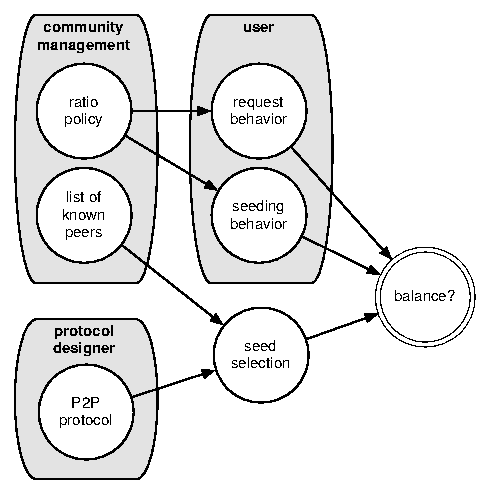
\includegraphics[width=0.7\textwidth]{pics/p2psys_balance.pdf}
	\caption{System properties and its relation to P2P balance \cite{2011:managesupplydemand:meulpolder}.}.
	\label{fig:sysbalance}
\end{figure}

% undersupply vs oversupply
In classical file-sharing peer-to-peer system, it is common to see that a swarm is \textit{undersupplied}. Undersupply means that there are not enough resource shared within the swarm to be distributed over the peers who wanted it. The reason why a user join a swarm is to download a file, so that is why undersupplied is commonly occurred. However, with the introduction of private community which enforce upload policy such as SRE or reputation mechanism, the problem shifted to a phenomenon called \textit{oversupply}. Both undersupply and oversupply is the sub-case of supply and demand misalignment. Undersupply condition can be solved by adding more high performance peer to boost download experience. In the other hand, oversupply problem is not trivial to solve.

% oversupply -> fierce upload competition -> unbalance situation
In oversupplied swarm, user may find it difficult to earn the credit by uploading the file. This is because the problem described by \citeauthor{2011:managesupplydemand:meulpolder} called ``upload competition'' \cite{2011:managesupplydemand:meulpolder}. Two conditions from peers perspective must be fulfilled to make P2P system sustain, which is peers must be cooperative, and cooperative peer must stay as long as possible in the swarm \cite{2011:managesupplydemand:meulpolder}. In upload competition problem, cooperative peer can not control his upload rate. The one who will download the seeder chunks is out of the seeder knowledge and control. This may result an expulsion from the community with a SRE because the cooperative peer looks like it do not contribute. \citeauthor{2010:crashsustain:rahman} also stated that oversupply may result to system seize up by \textit{crashing}  \cite{2010:crashsustain:rahman}. Sustainability of a swarm is in a risk in this situation.

% balance -> not sustain
\citeauthor{2011:managesupplydemand:meulpolder} in his work illustrated the relation between various P2P system properties and its relation to system balance. The illustration shown in figure \ref{fig:sysbalance}. Request and seeding behavior is another term of user downloading and uploading behavior, respectively. Seed selection is one part that responsible for choosing which peer to seed. In \cite{2011:managesupplydemand:meulpolder}, \citeauthor{2011:managesupplydemand:meulpolder} showed that using naive random seeding behavior is not sufficient to make P2P system balance. Unbalance system can lead to unsustainable community. Therefore, it is important to work study seeding behavior for each peer by the implementation of credit mining.

\section{Document Structure}
\todo{may be changed}
This thesis is structured as follows. Chapter 2 discusses problem we intend to solve and related work of it. Chapter 3 presents the design of credit mining system integrated with Tribler. Implementation of the mechanism and it's experiment will be elaborated in chapter 4. Chapter 5 shows performance of credit mining system. At the end, chapter 6 concludes the work mentioning possible future work.


